\documentclass[12pt,aspectratio=169]{beamer}

\usetheme[progressbar=frametitle]{metropolis}
\usepackage{appendixnumberbeamer}
\usepackage{booktabs}
\usepackage[scale=2]{ccicons}

\usepackage{pgfplots}
\usepgfplotslibrary{dateplot}

\usepackage{xspace}
	%\definecolor{almond}{rgb}{0.94, 0.87, 0.8}
		\definecolor{cornsilk}{rgb}{1.0, 0.97, 0.86}
%\definecolor{Purple}{HTML}{911146}
%	\definecolor{coolblack}{rgb}{0.0, 0.18, 0.39}
%\setbeamercolor{frametitle}{bg=coolblack}
	%\definecolor{burgundy}{rgb}{0.5, 0.0, 0.13}
	%\definecolor{bluep}{rgb}{0.2, 0.2, 0.6}
		\definecolor{darkslateblue}{rgb}{0.28, 0.24, 0.55}
%\definecolor{vsplblue}{HTML}{00a1e5}
%\setbeamercolor*{palette primary}{fg=vsplblue!60!black,bg=gray!30!white}
%\setbeamercolor{titlelike}{fg=darkslateblue}
\setbeamercolor{frametitle}{fg=prussianblue,bg=white}
%\definecolor{vsplbggray}{HTML}{efefef}
\definecolor{ivory}{rgb}{1.0, 1.0, 0.94}
	\definecolor{junglegreen}{rgb}{0.16, 0.67, 0.53}
		\definecolor{persiangreen}{rgb}{0.0, 0.65, 0.58}
\setbeamercolor{progress bar}{fg=persiangreen}
\setbeamercolor{alerted text}{fg=persiangreen}
%\definecolor{myteal}{HTML}{44AA99}
	%\definecolor{darkslateblue}{rgb}{0.28, 0.24, 0.55}
%\definecolor{myred}{HTML}{661100}
%\setbeamercolor{background canvas}{bg=red}
	\definecolor{prussianblue}{rgb}{0.0, 0.19, 0.33}
	\definecolor{gray}{rgb}{0.5, 0.5, 0.5}
%% This is pretty good; tan, seagreen, dark blue
	%	\definecolor{darkslateblue}{rgb}{0.28, 0.24, 0.55}
%\definecolor{ivory}{rgb}{1.0, 1.0, 0.94}
	%\definecolor{junglegreen}{rgb}{0.16, 0.67, 0.53}
	%	\definecolor{persiangreen}{rgb}{0.0, 0.65, 0.58}
		\definecolor{slategray}{rgb}{0.44, 0.5, 0.56}
%\setbeamercolor{progress bar}{fg=persiangreen}
%\setbeamercolor{titlelike}{fg=darkslateblue}
%\setbeamercolor{frametitle}{fg=darkslateblue,bg=ivory}


\setbeamercolor{titlelike}{fg=white}
%\setsansfont[BoldFont={Fira Sans SemiBold}]{Fira Sans Book}

\title{Bootstrapping Confidence Intervals \\ (with Confidence!)}
%\subtitle{A modern beamer theme}
% \date{\today}
\date{}
\author{Aaron Kaufman}
\institute{November 16, 2018}
	

\begin{document}

{\setbeamercolor{background canvas}{bg=prussianblue}
\setbeamercolor{normal text}{fg=white}
\maketitle
}

\setbeamercolor{normal text}{fg=gray}\usebeamercolor*{normal text}

\begin{frame}
\frametitle{Previously: Calculating Confidence Intervals}


\uncover<2->{\textbf{95\% Confidence Interval:} \uncover<3->{ If we construct 100 such intervals, 95\% will contain the truth}}

\uncover<4->{\textbf{Procedure:}}
\begin{enumerate}
	\item<5->{Calculate a quantity of interest, \textbf{X}}
	\item<6->{Calculate a standard deviation, \textbf{$s$}}
	\item<7->{Calculate a standard \textbf{error} \textbf{$\sigma$}: $\frac{s}{\sqrt{n}}$} 
	\item<8->{Use a Z-table to figure out how many SEs you need \uncover<9->{(1.96 for 95\%, 2.58 for 99\%)}}
	\item<10->{For 95\%: $[X - 1.96 \times \sigma, X + 1.96 \times \sigma]$}
\end{enumerate}

\end{frame}

%% We know how to calculate a confidence interval using the normal distribution, and what they're used for. 
%% We find the standard deviation of our estimate, maybe an average, calculate the standard deviation, and if we want a 95\% confidence interval, multiply by about 1.96, then our confidence intervial is our average +/- 1.96 * SD. 

\begin{frame}
\frametitle{Previously: Calculating Confidence Intervals}

\textbf{Example: \uncover<2->{What percentage of adult US citizens are registered to vote?}}
\uncover<3->{\textbf{Data:} \uncover<4->{2016 American National Election Study (4,142 US adults)}}

\begin{enumerate}
	\item<5->{\textbf{Average:} 85.7\%}
	\item<6->{\textbf{Standard Deviation:} 35.0\%}
	\item<7->{\textbf{Standard Error:} $\frac{34.9}{\sqrt{4,142}} = $ 0.5\%}
	\item<8->{\textbf{95\% Confidence Interval:} $[85.8 - 1.96\times 0.5, 85.8 + 1.96\times 0.5] = $ [84.6\%, 86.8\%]}
\end{enumerate} 

\uncover<9->{\textbf{Interpretation?}}
\uncover<10->{If we take 100 samples of 4,142 voters and construct 95\% CIs, then 95\% of them will contain the true percentage of (self-reported) registered voters}

\end{frame}

%% What this gives us is a way to quantify the uncertainty around our average. Where does this uncertainty come from? It comes from the fact that we don't have ALL the data, we only have a sample.

\begin{frame}
\frametitle{Why does this work?}

\uncover<2->{If a (representative) sample statistic has a 95\% chance of being within 1 margin of error of the true parameter...}

\uncover<3->{...then we are 95\% confident that the true parameter is within 1 margin of error of our sample statistic!}



% Verbally: Sometimes there is more than one source of randomness! And sometimes we don't know for sure. Sometimes it's the treatment assignment, and sometimes it's the potential outcomes.

% So sometimes this analytic CI interval will fail! When might that be? When the sample isn't representative of the population! 
% It isn't the normal distributional assumption -- the sampling distribution of the sample mean is always normal under the Central Limit Theorem

\end{frame}



%% But we can't always do this. Not only do we want to avoid math if we can, but sometimes we have more complicated things we want confidence intervals for and we can't simply assume a normal distribution. 
%% So a simple solution to calculating confidence intervals is called the bootstrap. 
%% In very broad strokes, the gyst of the bootstrap is that we take the data we have and we resample it WITH REPLACEMENT. Then we perform all our subsequent analyses, and we get a DISTRIBUTION of possible results. 
%% The theory here is that our data comes from a hypothetical population of data, if we were to take ANOTHER SAMPLE from that population, we could get another ``draw'' for our quantity of interest. 

\begin{frame}
\frametitle{An Alternative Approach: The Bootstrap}

\textbf{Why Bootstrap?}
\begin{itemize}
	\item<2-> Doing less math is better % The math is easy above, but it gets much harder quickly
	\item<3-> Sometimes the math won't work % Sometimes the process we'd like a CI for is really really complicated
\end{itemize}

\uncover<4->{\textbf{Bootstrap:} \uncover<5->{A computational solution to confidence intervals \uncover<6->{(much less math)}}}

\begin{enumerate}
	\item<7->{\textbf{Resample:}\uncover<8->{ resample the original data \textit{with replacement}}}
	\item<9->{\textbf{Recalculate:}\uncover<10->{ recalculate the original statistic of interest \textit{for each resample}}}
	\item<11->{\textbf{Find Quantiles:}\uncover<12->{ take the 2.5\% and 97.5\% quantiles of the bootstrapped statistics}}
\end{enumerate}

\end{frame}



{\setbeamercolor{background canvas}{bg=white!20}
\begin{frame}
\frametitle{The Bootstrap: Terminology}

\centering
\only<2>{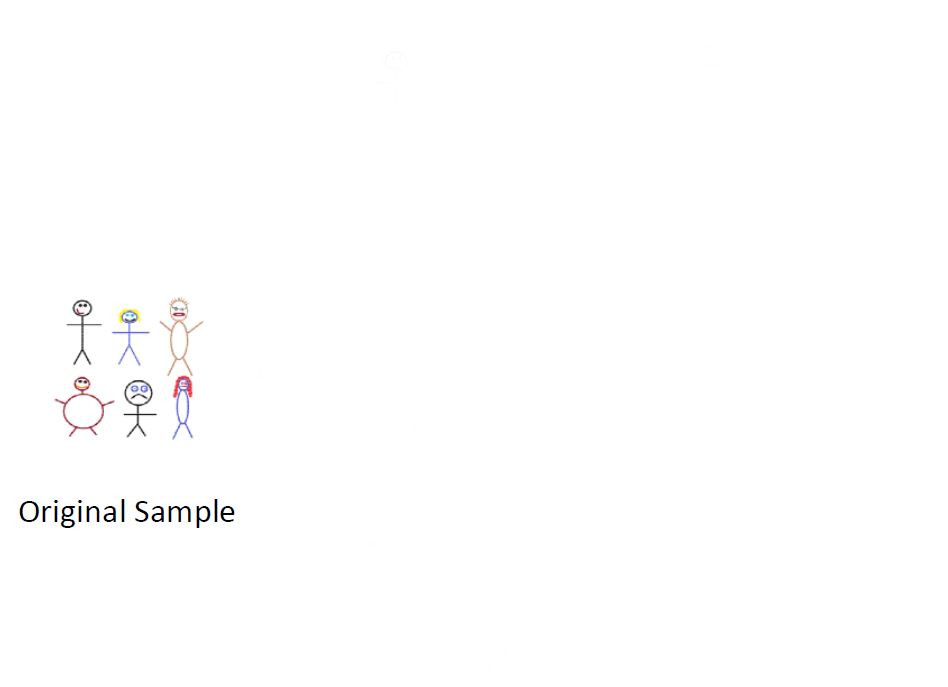
\includegraphics[width=.75\textwidth]{sample1.JPG}}
\only<3>{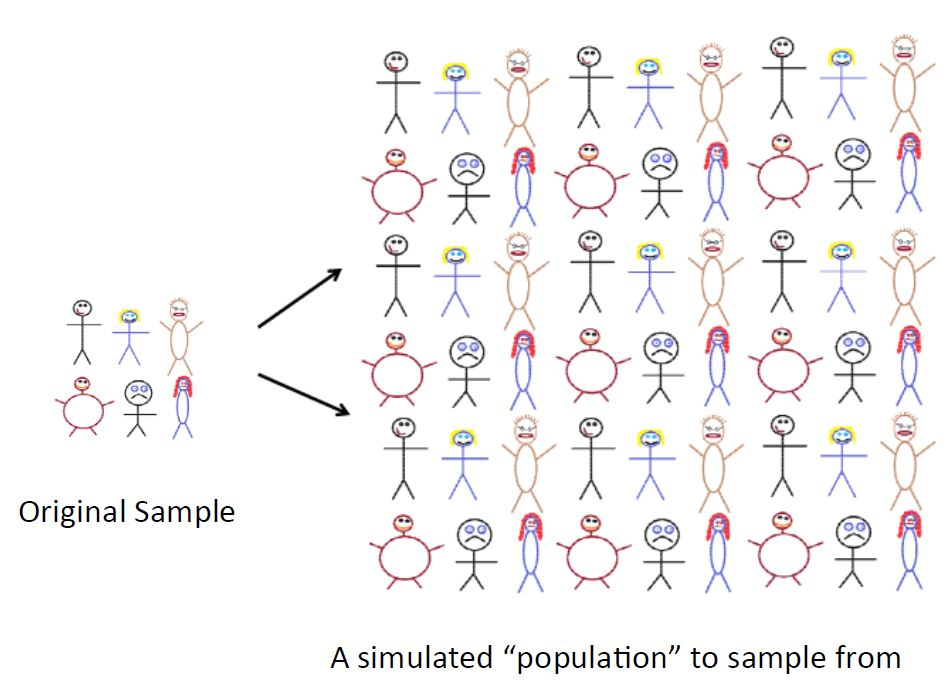
\includegraphics[width=.75\textwidth]{sample2.JPG}}
\only<4>{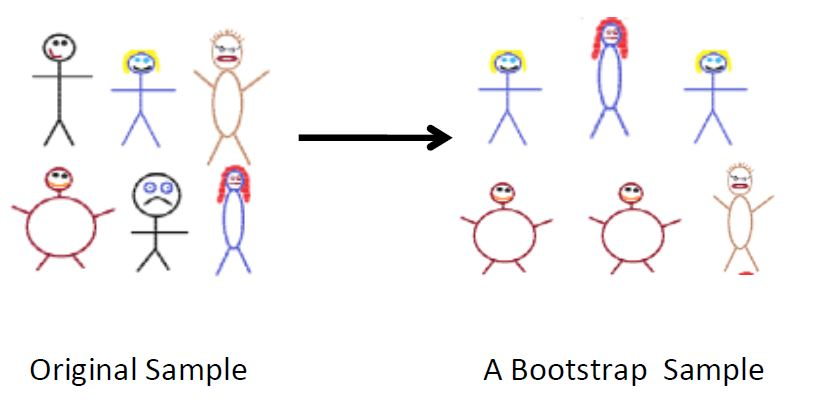
\includegraphics[width=.75\textwidth]{sample3.JPG}}
\only<5>{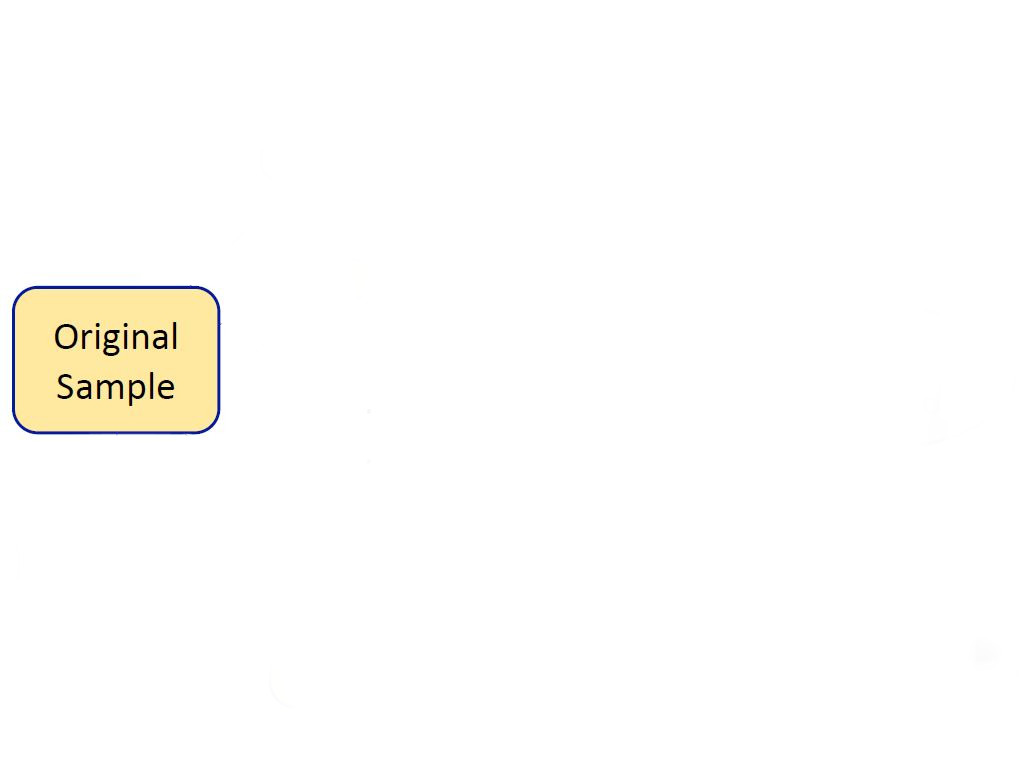
\includegraphics[width=.75\textwidth]{flowchart1.JPG}}
\only<6>{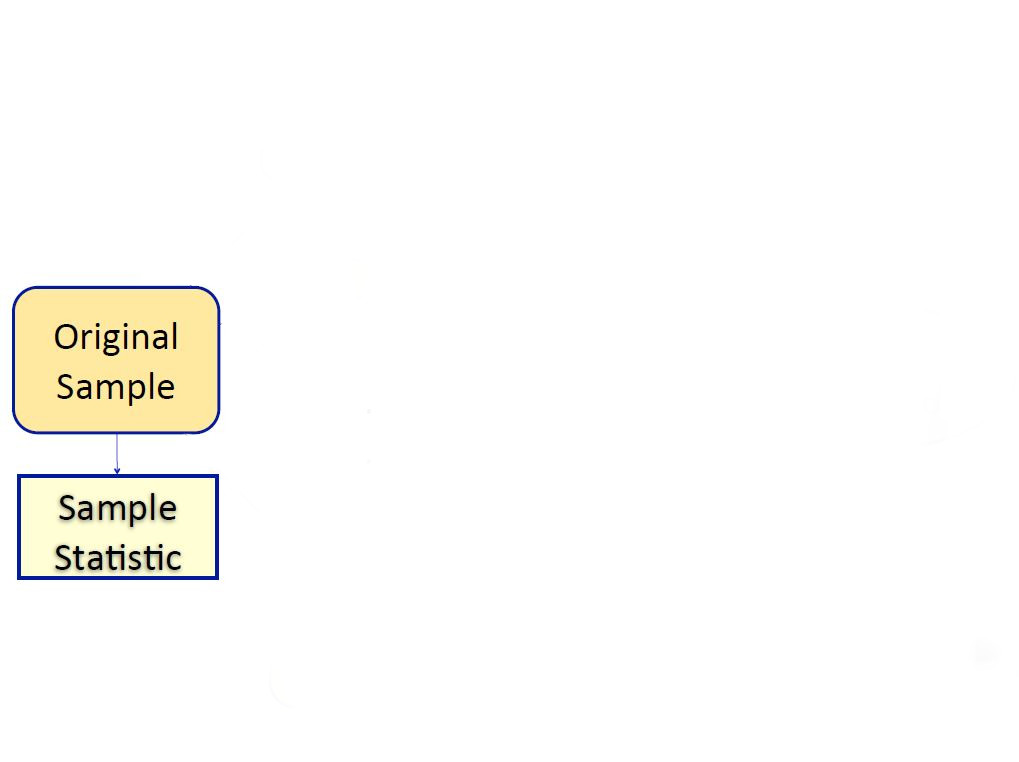
\includegraphics[width=.75\textwidth]{flowchart2.JPG}}
\only<7>{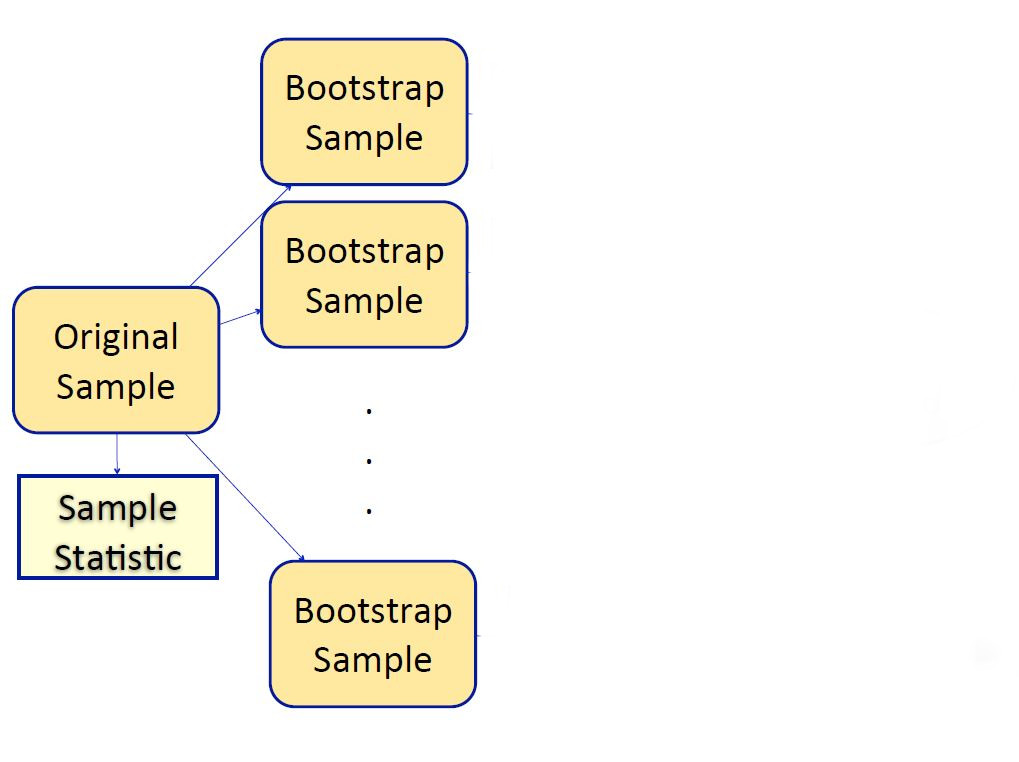
\includegraphics[width=.75\textwidth]{flowchart3.JPG}}
\only<8>{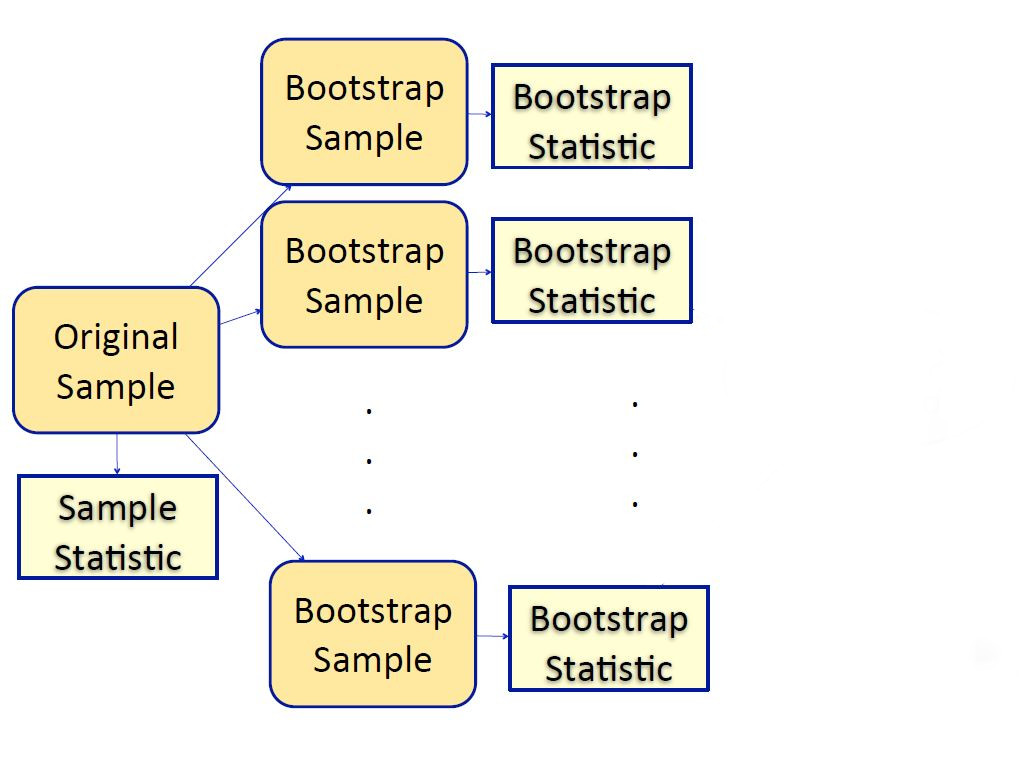
\includegraphics[width=.75\textwidth]{flowchart4.JPG}}
\only<9>{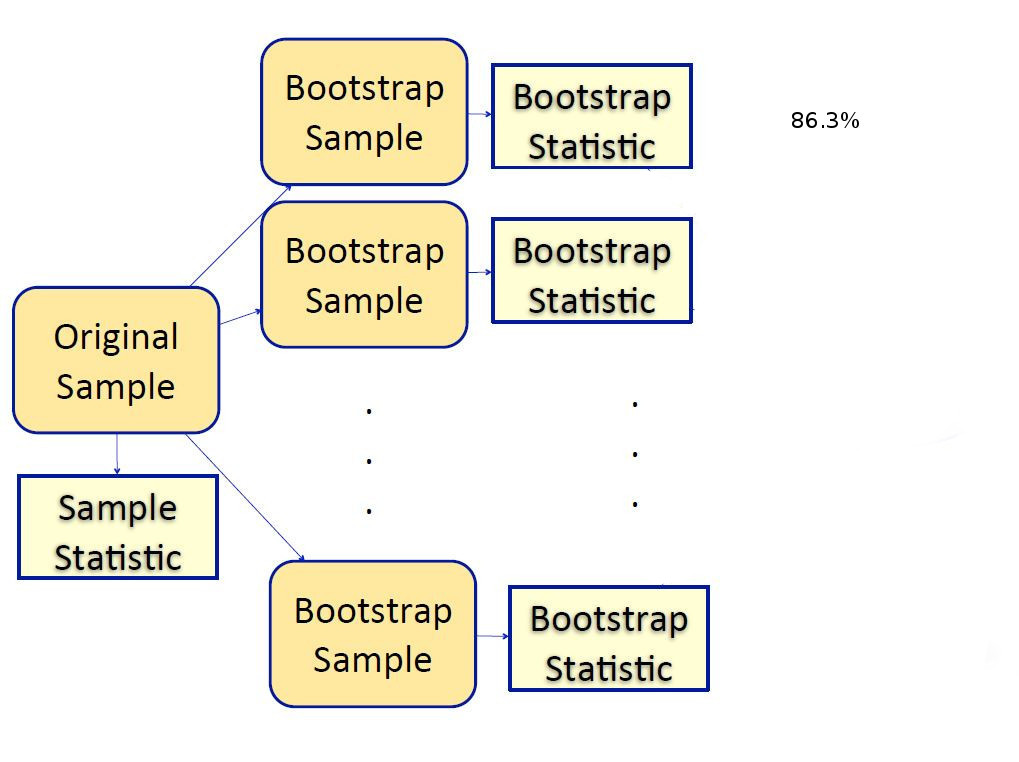
\includegraphics[width=.75\textwidth]{flowchart5.JPG}}



\end{frame}
}


%[Move to R Studio]
%% Here is a big political science data set in R Studio.
%% If we wanted to calculate the turnout rate in our sample, we could do it the analytic way:
%% Take the mean of the variable identifying voter turnout, calculate the SD, then construct the interval. 
%% But we could also do it with the bootstrap:
%% We sample our data with replacement 100 times, and get a VECTOR of potential turnout rates. Then we can take the 0.025 and 0.975 quantiles of this distribution (so that 95\% of the data are in the middle), and that's ANOTHER approach to calculate a confidence interval, no math required.



%% But we can use the bootstrap for more than just averages too!

%% Here is what it looks like it we try to visualize the relationship between age and turnout:
%% As you've already learned, we could quantify this relationship using a regression, and get a confidence interval from that regression.
% [regression here]
%% But you may not know that the regression calculates its standard errors using lots of matrix algebra and partial derivates, which we'd REALLY like to not have to do.
%% But you can bootstrap that too!

%% Here's how we do it: we sample the data set, and each time, we run the regression and extract the coefficient.
%% Then, same as before, we can take the quantiles of that distribution and get a confidence interval!


%% Summary slide:
% 1) The bootstrap is a computational approach when analytic approaches fail (or we just don't want to use them)
% 2) It involves resampling our full data set WITH REPLACEMENT, then calculating our QOI
% 3) It makes it easier to calculate confidence intervals of different confidences (90, 95, 99.9999, etc)
% 4) It works for complicated stuff too! [Example from my work]

% Some coding tips when doing this:
% 1) The mosaic R package includes the shuffle() function: shuffle(dat, replace=FALSE)
% 2) The replicate() function repeats a snippet of code however many times you want
% 3) calculate quantiles: quantile(bootstrapped.avgs, c(0.025, 0.975))

\begin{frame}
\frametitle{R Coding: The American National Election Study}


\end{frame}


\begin{frame}
\frametitle{Summary \& Coding tips}

\uncover<2->{\textbf{The bootstrap...}}
\begin{enumerate}
	\item<3->{Is useful when analytic approaches fail (or when we are feeling lazy)}
	\item<4->{Involves resampling the full data \alert{with replacement}}
	\item<5->{Works for complicated sample statistics too}
\end{enumerate}

\uncover<6->{\textbf{To make it easier...}}
\begin{itemize}
	\item<7->{Use the \texttt{replicate()} function to repeat your resampling lots of times}
	\item<8->{Use the \texttt{shuffle()} function from the \texttt{mosaic} library: \uncover<9->{\texttt{mosaic::shuffle(dat, replace=FALSE)}}}
	\item<10->{Calculate quantiles: \uncover<11->{\texttt{quantile(bootstrapped.avgs, c(0.025, 0.975))}}}
\end{itemize}
\end{frame}

%% Wrap up frame with a link to the code here

\begin{frame}
\frametitle{Thank you!}

\textbf{\LaTeX, R code, and data at:} \\
\vspace{.2in}
\url{http://www.github.com/aaronrkaufman/bootstrap}


\end{frame}


\end{document}


%%% Talk about how it fails over the support